% !TeX encoding = UTF-8
% !TeX spellcheck = en_US
% !TeX root = ../../Thesis.tex

\chapter{Vacuum test chamber}
\label{ch:Vacuum chamber}

\textcolor{red}{ignore from here} \\
2020-08-30 leak rate
2020-09-27 set voltages
2020-09-30 first successful external run
2020-10-07 spot vs pressure
2020-10-22 current measurement aluminum foil
2020-11-05 forgot to turn off filament heating
2020-11-14 assemble chamber with copper rings \\
\textcolor{red}{to here}

In order to be able to fit the CRT screen, CF160 flanges were chosen for the test chamber. At one point during testing, major changes were made which will be explained in \cref{sec:Second iteration}.

\section{First iteration}
\label{sec:vacuum chamber first iteration}

A 3D render of the chamber is shown in  (\cref{fig:3D rendering of test chamber}). Without a CRT installed, it was possible to reach a pressure of \SI{6.8e-7}{\milli\bar}, while with one the lowest was \SI{2.0e-6}{\milli\bar}.
 
\subsection{Parts}
\label{subsec:Parts}
 
The center piece consists of a 6-way cross with view ports at the front and bottom. A valve was installed at the back in order to flood the chamber with nitrogen\todo{pure nitrogen name?} when installing a new CRT to avoid oxygen poisoning. On the right side, a HiCube 300 Eco turbo pump was installed and on the left side a wobble stick was attached with a wire. A nipple fitting \todo{length} was installed at the top with a 5 port cluster flange, each being of type CF63.
 
In the middle port, a VSH vacuum transducer was installed to measure pressure. This needs a \SI{24}{\volt} dc power supply. On the left, a 19 pin connector \todo{how many pins and model name?} was installed to supply the necessary voltages to the CRT. Two flanges were equipped with four BNC feedthroughs each. One of them was used to connect do the x-, and y-plates, while the other connected to the wobble stick and aluminum foil at the CRT screen. Further explanation will be given in \todo{ref ch:Beam characterization, include picture there}. The last port was capped off by a blank flange.
 
For the inside wires, stranded copper cables were used. The chamber was sealed by rubber gaskets.
 
\begin{figure}[ht]
	\centering
 	
	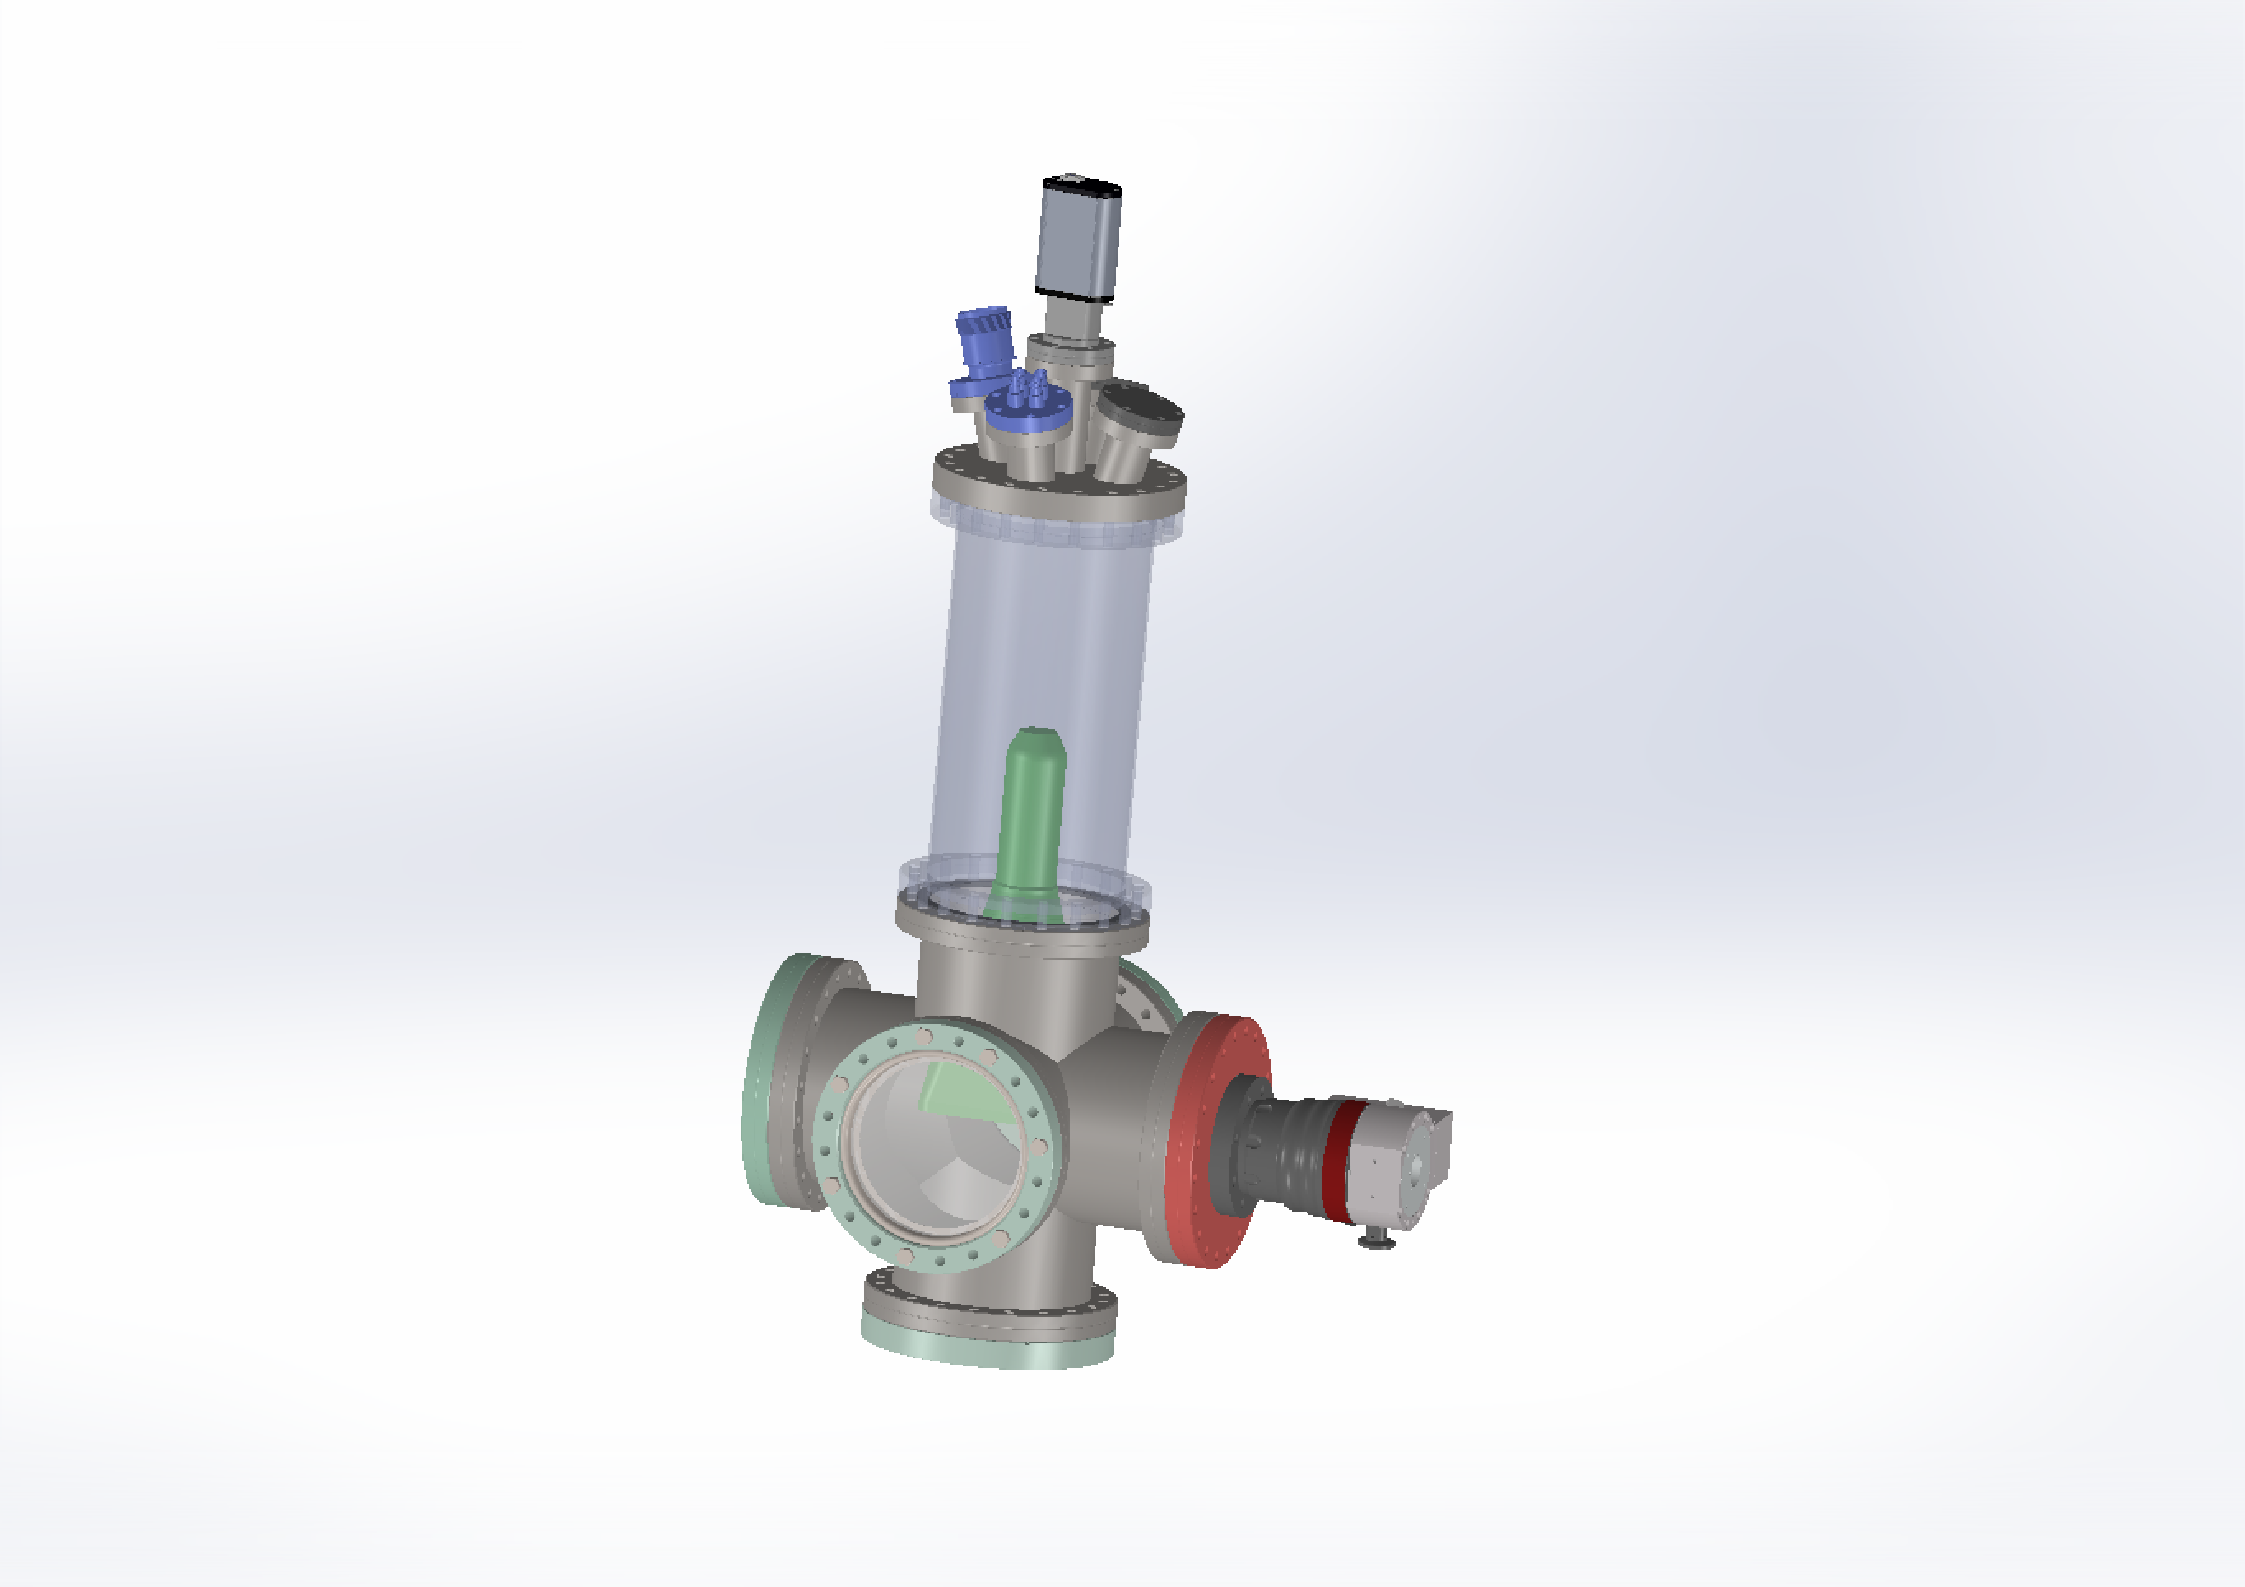
\includegraphics[width=0.9\textwidth]{./Chapters/vacuum-chamber/test_chamber} % taken from OneNote QuaK/Vacuum Setup/Test vacuum chamber
	
	\caption{3D rendering of test chamber.}
	\label{fig:3D rendering of test chamber}
\end{figure}
 
\subsection{CRT mounting mechanism}
\label{subsec:CRT mounting mechanism}

 Two M8 rods of length \todo{rod length?} were drilled into the cluster flange. On each, a L-piece was installed between two nuts and they were connected by a hose clamp. Two of these were used to secure the CRT inside the nipple facing the cross (\cref{fig:Image of CRT mounting mechanism}).
 

\begin{figure}[h]
	\centering
	
	\missingfigure[figwidth=0.9\textwidth]{Image of CRT mounting mechanism.}
	
	\caption{Image of CRT mounting mechanism.}
	\label{fig:Image of CRT mounting mechanism}
\end{figure}


\subsection{Leak test}
\label{subsec:Leak test}

Before inserting a CRT, a leak test was performed. First, the chamber was set to a pressure of \SI{e-5}{\milli\bar} after which the pump was turned off. The pressure was measured once a minute for a duration \SI{3}{\hour}. This is shown in \cref{fig:Leak rate of test chamber after turning off pump}.

\begin{figure}[ht]
	\centering
		
	\begin{tikzpicture}
		% !TeX encoding = UTF-8
% !TeX spellcheck = en_US
% !TeX root = ../../Thesis.tex

\begin{axis}[
	%name=zeemanShift,
	%grid=major,
	ymode = log,
	xlabel = time/\si{\minute},
	ylabel = pressure/\si{\milli\bar},
	%scaled ticks=false,
	%		every x tick scale label/.style={at={(xticklabel* cs:1.03,-0.3em)}, /pgfplots/near ticklabel align=outside, anchor=near xticklabel opposite, inner sep=0pt},
	%		xticklabel style={/pgf/number format/sci}, sci generic={mantissa sep=\cdot,exponent={10^{#1}}}},
	%yticklabel style={/pgf/number format/sci},
	xmin = 0,
	ymin = 1e-5,
	%extra tick style={grid=none}, 
	%width=0.7\textwidth,
	%legend style={at={(1.02, 0.5)}, anchor = west},
	%every axis plot/.append style={thick}
	]
	\addplot[mark=none, black] table [x=t, y=p, col sep=comma]{./Chapters/vacuum-chamber/leak_rate.csv};
\end{axis}
	\end{tikzpicture}
	
	\caption{Leak rate of test chamber after turning off pump.}
	\label{fig:Leak rate of test chamber after turning off pump}
\end{figure}


\section{Second iteration}
\label{sec:Second iteration}

At one point during experimentation, major changes were made to the chamber. Thanks to these, it was possible to reach a pressure of \SI{1.2e-7}{\milli\bar}.

\subsection{Changes}
\label{subsec:Changes}

First, every rubber gasket was changed to a copper one for a better seal, except at the cluster flange, since that spot will be opened and closed the most often. Each copper stranded cable inside was switched to a coaxial one and the mantle was connected to the chamber wall, which was set to ground. A Faraday cup was installed below the wobble stick, to accurately measure the beam current (further details in \todo{ref ch:Beam characterization}). The aluminum foil was extended to cover all four sides of the screen.

\subsection{Fastening}
\label{subsec:Fastening}

When attaching flanges, it is important to start with a low torque and to fasten opposite screws to prevent too much force on one side of the gasket. For M6 screws, the torque was incrementally set to \SIlist{6;10;15;20}{\newton\meter} and for M8 screws \SIlist{8;16;25}{\newton\meter}. After finishing every opposite screw pair at a set torque, the procedure was repeated twice before going to a higher torque. This was done in order guarantee a tight and even seal.